\documentclass[crop,tikz]{standalone}

\usepackage[utf8]{inputenc}

% 'crop' is the default for v1.0, before it was 'preview'
%\usetikzlibrary{...}% tikz package already loaded by 'tikz' option
\usetikzlibrary{arrows} 

\begin{document}

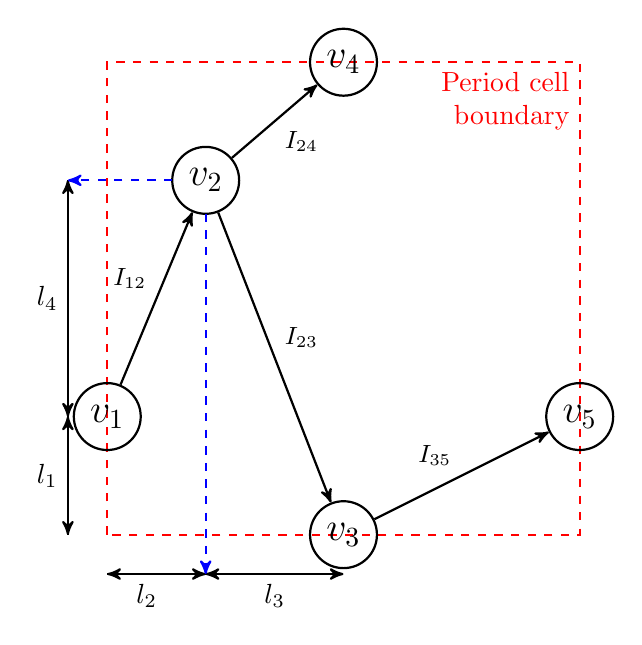
\begin{tikzpicture}[->,>=stealth',auto,node distance=3cm,thick,main node/.style={circle,draw,font=\sffamily\Large\bfseries}]

	%periodic boundary, unit cell boundary
	\draw[dashed, red] (-3cm,-3cm) rectangle (3cm,3cm);
	\node[anchor=north east, align=right, red] at (3cm,3cm) {Period cell \\ boundary};
	
	%nodes
	\node[main node] (1) at (-3,-1.5) {$v_1$};
	\node[main node] (2) at (-1.75,1.5) {$v_2$};
	\node[main node] (3) at (0,-3) {$v_3$};
	\node[main node] (4) at (0,3) {$v_4$};
	\node[main node] (5) at (3,-1.5) {$v_5$};
	
	%edges
	\path[every node/.style={font=\sffamily\small}]
		(1) edge node[anchor=south east] {$I_{12}$} (2)
		(2) edge node[anchor=north west] {$I_{24}$} (4)
		(2) edge node[anchor=south west] {$I_{23}$} (3)
		(3) edge node[anchor=south east] {$I_{35}$} (5);
	
	%varying lengths of things
	\draw[->] (-3.5, -3) -- (-3.5,-1.5);
	\draw[->] (-3.5,-1.5) -- (-3.5, -3);
	\node[anchor=east] at (-3.5,-2.25) {$l_1$};
	\draw[->] (-3, -3.5) -- (-1.75, -3.5);
	\draw[->] (-1.75, -3.5) -- (-3, -3.5);
	\node[anchor=north] at (-2.5, -3.5) {$l_2$};
	\draw[->] (-1.75, -3.5) -- (0, -3.5);
	\draw[->] (0, -3.5) -- (-1.75, -3.5);
	\node[anchor=north] at (-0.875, -3.5) {$l_3$};
	\draw[->] (-3.5, -1.5) -- (-3.5, 1.5);
	\draw[->] (-3.5, 1.5) -- (-3.5, -1.5);
	\node[anchor=east] at (-3.5, 0) {$l_4$};
	
	%wireframes for ease of sight
	\draw[dashed, blue] (-1.75, 1.075) -- (-1.75, -3.5);
	\draw[dashed, blue] (-2.175, 1.5) -- (-3.5, 1.5);
	
\end{tikzpicture}

\end{document}